% Figures for the update (analyze/update_figures.py). Needs \usepackage{graphicx}.
\begin{figure}[H]
    \centering
    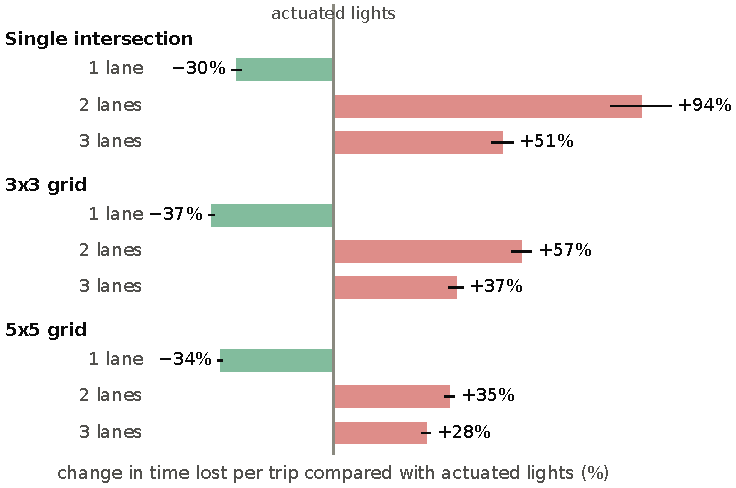
\includegraphics[width=\linewidth]{carma_vs_actuated.pdf}
    \caption{Carma cuts time lost per trip by 30--37\% against
    actuated lights on one-lane roads, and increases it by 28--94\% on
    two- and three-lane roads. Learned bids, reference setting (moderate demand, 6 trips per driver,
    20\% urgent trips, lane bids, 80 starting carma), 7-day evaluation week; bars are means of
    10 seeds (green: less time lost than actuated lights, red: more), whiskers 95\%
    intervals across seeds.}
    \label{fig:carma_vs_actuated}
\end{figure}

\begin{figure}[H]
    \centering
    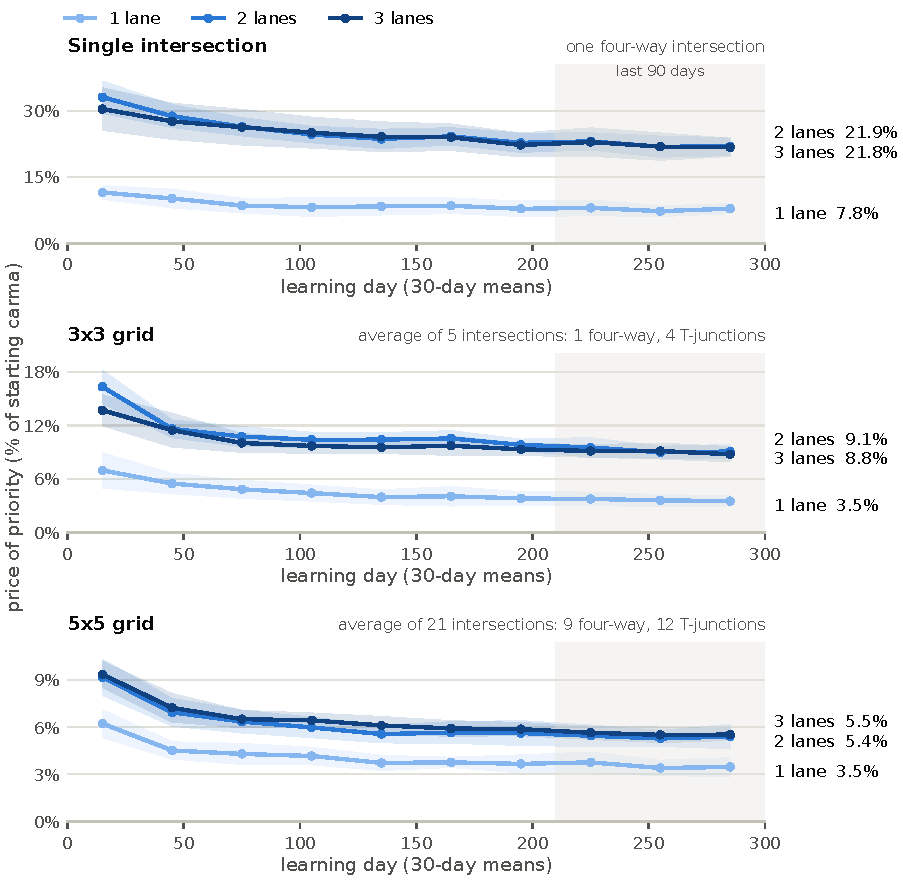
\includegraphics[width=\linewidth]{learned_price_300_days.pdf}
    \caption{The learned price of priority falls 29--50\% from the first to the last
    month of 300 learning days. The fall slows from 9--29\% between the first and
    second months to at most 3\% a month over the last 90 days; on the grids it has not
    quite stopped. Median winning bid in contested auctions as a share of starting carma, single intersection, 3x3 grid and 5x5 grid;
    each grid's value is the unweighted mean over its signalised intersections (5 on the 3x3: 1
    four-way and 4 T-junctions; 21 on the 5x5: 9 four-way and 12 T-junctions; the corners are
    bends without auctions). Reference setting, 30-day means of 10 seeds with 95\% bands; shaded: the last 90 days;
    labels: the last 30 days; each panel has its own y scale.}
    \label{fig:learned_price}
\end{figure}
